\documentclass[12pt]{article}
\usepackage{verbatim}
\usepackage[dvips]{epsfig}
\usepackage{color}
\usepackage{url}
\usepackage[colorlinks=true]{hyperref}

\begin{document}

\section*{GENESIS: Documentation}

{\bf Related Documentation:}
% start: userdocs-tag-replace-items related-do-nothing
% end: userdocs-tag-replace-items related-do-nothing

\subsection*{Figure\,11}

\begin{figure}[h]
\centering
   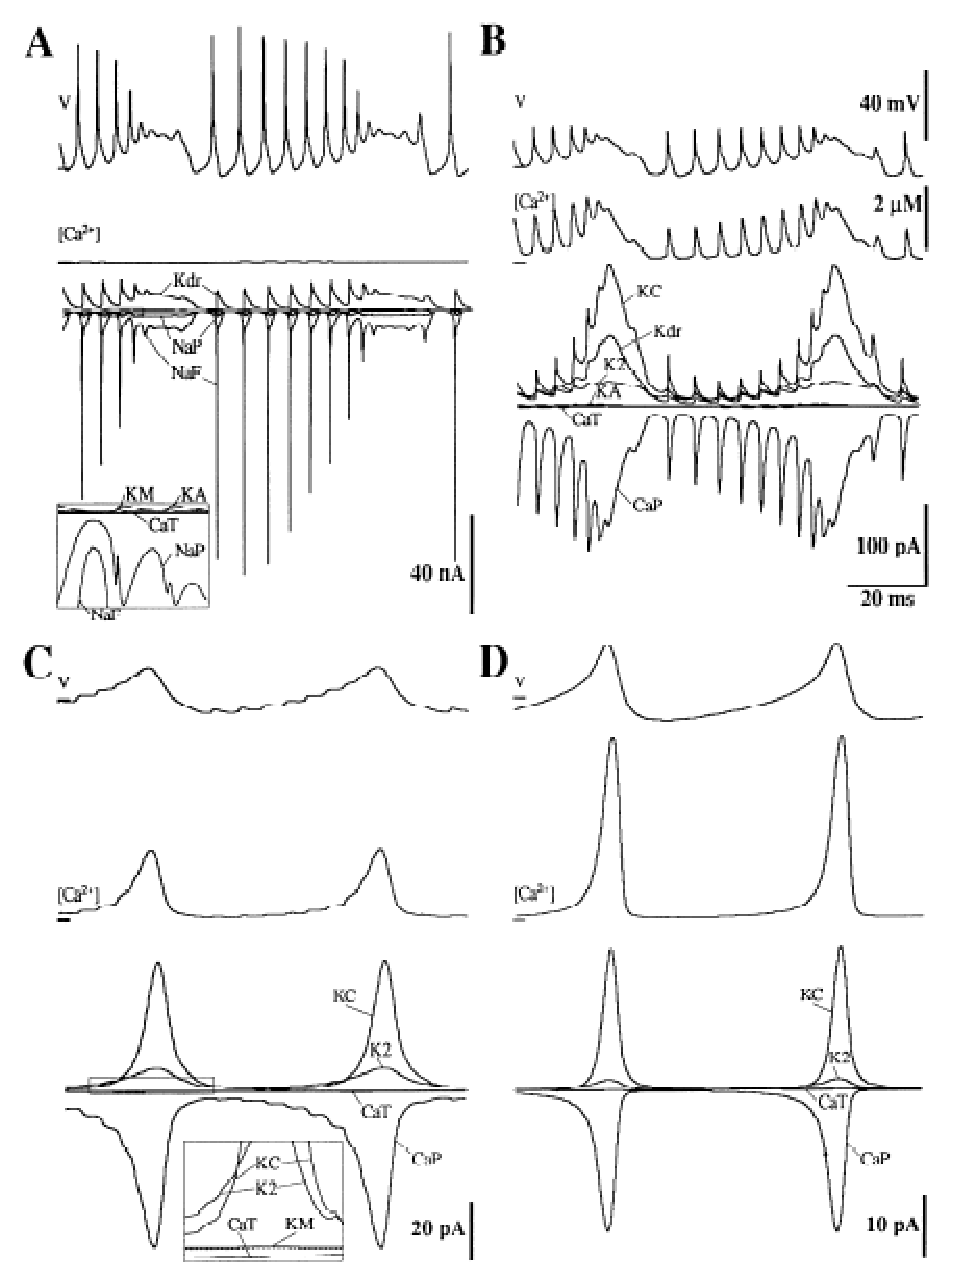
\includegraphics[scale=1]{figures/Fig.1.11.eps}
   \caption{Dynamic change in model variables during somatic and dendritic spikes. The same 100\,ms sequence is shown at 4 representative locations in the model during a 2.0\,nA current injection in the soma, 900\,ms after the start of the current injection (model PM9). {\it A}: Soma. {\it B}: Main dendrite. {\it C}: Smooth dendrite. {\it D}: Spiny dendrite. Each part of the figure shows the membrane potential (V, {\em top trace}), the Ca$^{2+}$ concentration ([Ca$^{2+}$], {\em middle trace}), and the amplitude of all ionic currents ({\em superimposed bottom traces}) in the compartment. {\it A} and {\it C}: Part of the current traces enlarged in a small box. The scale bars for voltage and concentration are identical in all sections. For the ionic currents each section is scaled differently (outward currents upward). Horizontal bar at {\em left} of V traces: -50\,mV membrane potential. Horizontal bar at {\em left} of [Ca$^{2+}$] traces: 0\,$\mu$M concentration. See \href{../pub-purkinje-deschutter1-table-1/pub-purkinje-deschutter1-table-1.tex}{\bf Table\,1} for abbreviations.}
   \label{fig:DS1.11}
\end{figure}

\bibliographystyle{plain}
\bibliography{../tex/bib/g3-refs.bib}

\end{document}
